\section{eo\-Stoch\-Tournament\-Select$<$ EOT $>$ Class Template Reference}
\label{classeo_stoch_tournament_select}\index{eoStochTournamentSelect@{eoStochTournamentSelect}}
eo\-Stoch\-Tournament\-Select: a selection method that selects ONE individual by binary stochastic tournament -MS- 24/10/99  


{\tt \#include $<$eo\-Stoch\-Tournament\-Select.h$>$}

Inheritance diagram for eo\-Stoch\-Tournament\-Select$<$ EOT $>$::\begin{figure}[H]
\begin{center}
\leavevmode
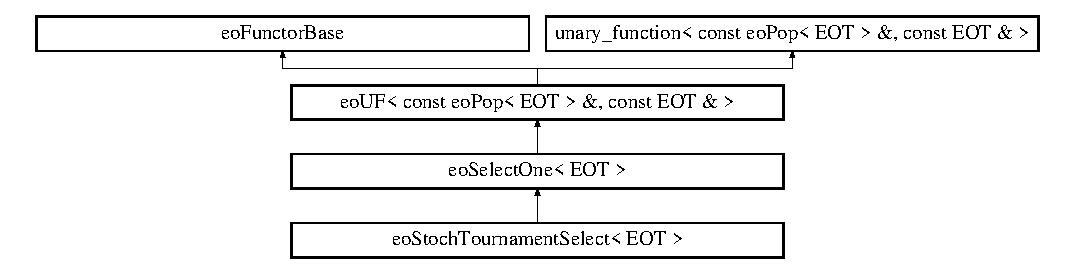
\includegraphics[height=3.23699cm]{classeo_stoch_tournament_select}
\end{center}
\end{figure}
\subsection*{Public Member Functions}
\begin{CompactItemize}
\item 
{\bf eo\-Stoch\-Tournament\-Select} (double \_\-Trate=1.0)\label{classeo_stoch_tournament_select_a0}

\item 
virtual const {\bf EOT} \& {\bf operator()} (const {\bf eo\-Pop}$<$ {\bf EOT} $>$ \&pop)\label{classeo_stoch_tournament_select_a1}

\begin{CompactList}\small\item\em Perform the stochastic tournament. \item\end{CompactList}\end{CompactItemize}
\subsection*{Private Attributes}
\begin{CompactItemize}
\item 
double {\bf Trate}\label{classeo_stoch_tournament_select_r0}

\end{CompactItemize}


\subsection{Detailed Description}
\subsubsection*{template$<$class EOT$>$ class eo\-Stoch\-Tournament\-Select$<$ EOT $>$}

eo\-Stoch\-Tournament\-Select: a selection method that selects ONE individual by binary stochastic tournament -MS- 24/10/99 



Definition at line 42 of file eo\-Stoch\-Tournament\-Select.h.

The documentation for this class was generated from the following file:\begin{CompactItemize}
\item 
eo\-Stoch\-Tournament\-Select.h\end{CompactItemize}
